\subsection{Resultaatprotocol}
\label{result}

\begin{figure}[htpb]   
    \label{Figuur::recommendations}      
  \begin{center}    
 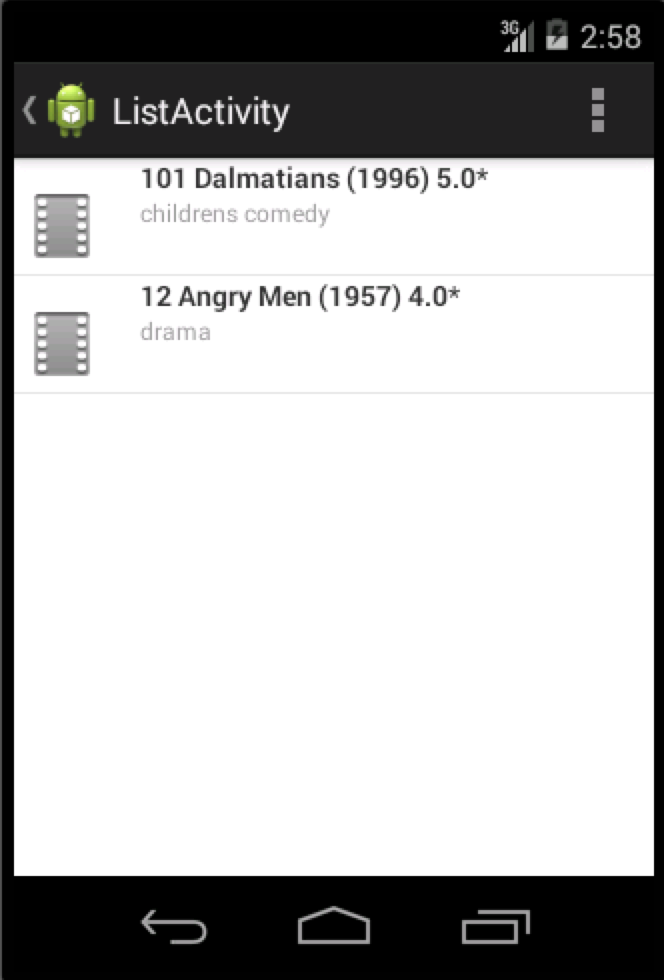
\includegraphics[scale=0.5]{fig/recommendations}    
  \end{center}   
  \caption{De gebruiker krijgt een lijst met aanbevelingen en een voorspelling van het aantal sterren dat hij aan deze film zou geven.}  
   \end{figure}
   
Het resultaatprotocol zorgt ervoor dat de twee berekende waarden per item uit \ref{sumoverallusers}, de som der ratings en het aantal, op een privacyvriendelijke manier bij de aanvrager terechtkomen. Bij het aanvragen van aanbevelingen gaf de clientapplicatie randomwaarden mee. Deze worden bij de waarden geteld en naar de controleserver gestuurd die ze decrypteert en terugstuurt naar de recommender, die op zijn beurt ze gewoon teruggeeft aan de gebruiker. De gebruiker trekt er zijn gegenereerde randomwaarden van af en verkrijgt de originele waarden. Hierop bepaalt hij de gemiddelde rating van gelijkaardige gebruikers door ze eenvoudigweg te delen. De clientapplicatie is wel verantwoordelijk om de items die reeds door de gebruiker zelf zijn beoordeeld uit de resultaten te filteren.
